% =====================================================================
% main.tex - Entrega 1 PLN: corpus, idea de proyecto y textometria
% Clase tg_usta (NO modificar tg_usta.cls). Compilar con pdflatex+bibtex.
% =====================================================================
\documentclass[11pt]{tg_usta}

\usepackage[utf8]{inputenc}
\usepackage[T1]{fontenc}
\usepackage{anysize}
\usepackage{graphicx}
\usepackage{subcaption}
\usepackage{booktabs}
\usepackage{url}

\marginsize{1in}{1in}{1in}{1in} %% Margenes de 1 pulgada (NO MODIFICAR)

% ---------------------------------------------------------------------
% Nota sobre las citas: tg_usta.cls carga el paquete `harvard', que
% redefine \cite y solo resuelve referencias de estilos propios
% (agsm/dcu). Para poder usar el estilo apalike (pedido en la guia de la
% entrega) se restaura aqui el \cite estandar del kernel de LaTeX, que
% resuelve las etiquetas \bibcite generadas por apalike.bst (formato
% [Autor, anio]). No se modifican las citas de harvard: simplemente se
% sustituye \cite por la definicion original del kernel.
\makeatletter
\renewcommand{\cite}{\@ifnextchar[{\@tempswatrue\@citex}{\@tempswafalse\@citex[]}}
\makeatother

\begin{document}

% =====================================================================
% PORTADA / ENCABEZADO
% =====================================================================
\title[maintitle = Análisis de sentencias de la Corte Constitucional de Colombia (1992--2021),
       secondtitle = {Entrega 1: corpus, idea de proyecto y textometría}]

\begin{authors}[Rivera, Carrillo, Garnica \& Prieto]

% Pontificia Universidad Javeriana, Bogotá (Colombia)
\author[firstname = Erika Valeria,
        surname = Rivera Jimenez,
        email = riveraev@javeriana.edu.co]

\author[firstname = Julian Guillermo,
        surname = Carrillo Meneses,
        email = carrillojuliang@javeriana.edu.co]

\author[firstname = Carlos Andres,
        surname = Garnica Salazar,
        email = carlos\_garnicas@javeriana.edu.co]

\author[firstname = Oscar Andres,
        surname = Prieto Moreno,
        email = o-prieto@javeriana.edu.co]

\end{authors}

\begin{center}\footnotesize Pontificia Universidad Javeriana, Bogotá, Colombia\end{center}

\begin{mainabstract}

Este proyecto explora computacionalmente un corpus de 23.742 sentencias de la Corte Constitucional de Colombia emitidas entre 1992 y 2021, construido a partir del repositorio público de Hugging Face \emph{Manuel/sentencias-corte-cons-colombia-1992-2021}. El documento presenta la idea de proyecto, la caracterización del corpus (fuente, formato, depuración y fragmentos representativos) y una textometría básica sobre la totalidad del corpus: limpieza y normalización del texto, medidas textuales globales, frecuencias léxicas con y sin palabras vacías, distribución temporal de las sentencias y nubes de palabras por año. Los resultados confirman el carácter extenso y formulaico del género ($\approx$ 11.000 palabras por documento) y el dominio del léxico jurídico-procesal una vez se eliminan las palabras funcionales ($\approx$ 48\,\% de los tokens). Esta caracterización sienta las bases para las siguientes entregas: lematización, representaciones vectoriales y clasificación automática.\\\\
\textit{\textbf{Palabras clave:}} procesamiento de lenguaje natural, lenguaje jurídico, Corte Constitucional de Colombia, corpus, textometría, análisis diacrónico.
\end{mainabstract}

% =====================================================================
% SECCION 1: IDEA DEL PROYECTO
% =====================================================================
\section{Idea del proyecto}

\subsection{Área de aplicación y dominio}
El proyecto se inscribe en el área del lenguaje jurídico: el análisis computacional de la jurisprudencia de la Corte Constitucional de Colombia mediante técnicas de procesamiento de lenguaje natural (PLN). Las providencias de esta corporación son documentos extensos (en promedio $\approx$ 11.000 palabras), con estructura discursiva formal (encabezado, antecedentes, consideraciones y parte resolutiva), terminología especializada, fórmulas de estilo estables y numerosas citas de normas y de jurisprudencia previa. El corpus comprende tres tipos de providencias: sentencias de tutela (T), de constitucionalidad (C) y de unificación (SU).

El arco temporal 1992--2021 habilita una segunda dimensión de análisis: la evolución del lenguaje de la Corte a lo largo de tres décadas. Como trabajo futuro se contempla enriquecer el análisis con lematización y etiquetado de categorías gramaticales (POS) mediante \emph{spaCy}, y explorar modelos de lenguaje preentrenados de dominio legal, del tipo LEGAL-BERT \cite{chalkidis2020legalbert}; estas técnicas no forman parte todavía de lo ejecutado, sino del horizonte del proyecto.

\subsection{Problema por abordar}
El problema central es de PLN aplicado: extraer conocimiento estructurado de un acervo textual enorme y sin metadatos. Cada sentencia es un documento largo en el que la información relevante (problema jurídico, hechos, decisión, regla) está dispersa entre fórmulas procesales repetidas, lo que dificulta su lectura, comparación y consulta manual. El corpus plantea, además, un desafío de representación: carece de anotaciones temáticas, y el tipo de providencia y el año de emisión deben inferirse del propio texto.

El proyecto aborda tres frentes: (i) caracterizar textométricamente el corpus; (ii) estudiar la evolución temporal del vocabulario y de los temas dominantes de la Corte; y (iii) explorar clasificación automática y resúmenes que faciliten la consulta de sentencias extensas.

\subsection{Justificación}
El análisis manual de decenas de miles de documentos largos es inviable; el PLN permite convertir ese contenido en evidencia cuantificable y reproducible. La literatura reciente documenta, además, la escasez de recursos y \emph{datasets} legales anotados en español para América Latina \cite{loffler2025predicting}, de modo que un corpus jurídico colombiano depurado y caracterizado textométricamente constituye en sí mismo un aporte. El proyecto puede apoyar la clasificación temática de decisiones, el seguimiento de la agenda de la Corte y la consulta de jurisprudencia, siempre como herramienta de apoyo a la interpretación especializada, no como sustituto.

\subsection{Preguntas de investigación}
\begin{itemize}
  \item ¿Qué propiedades léxicas y estilométricas caracterizan las sentencias y permiten diferenciar los tipos de providencia (T, C y SU) y los distintos periodos?
  \item ¿Cómo evoluciona el vocabulario de la Corte entre 1992 y 2021 en términos de riqueza léxica, términos dominantes y temas recurrentes?
  \item ¿Es posible clasificar automáticamente las sentencias según su tipo o su temática utilizando técnicas de PLN?
  \item ¿En qué medida pueden los métodos automáticos apoyar la consulta de sentencias extensas mediante resúmenes extractivos o abstractivos?
\end{itemize}

% =====================================================================
% SECCION 2: CORPUS
% =====================================================================
\section{Corpus: descripción y evidencia}

\subsection{Fuente del corpus}
El corpus proviene del repositorio abierto \emph{sentencias-corte-cons-colombia-1992-2021}, publicado por el usuario \emph{Manuel} en el Hugging Face Hub \cite{manuel2022sentencias}: \url{https://huggingface.co/datasets/Manuel/sentencias-corte-cons-colombia-1992-2021}, bajo licencia CC-BY-4.0. La descarga contiene un único archivo CSV de 1,68\,GB en UTF-8, denominado \texttt{Juris1992\_2022.csv}; el nombre del archivo es engañoso, pues la cobertura real es 1992--2021: no existen sentencias de 2022 y el año 2021 es parcial, con solo 20 documentos. La fuente primaria de los textos es la relatoría de la Corte Constitucional de Colombia.

\subsection{Características del corpus}
\begin{itemize}
  \item El CSV contiene 23.750 filas y dos columnas. Tras la depuración (sección 2.3) el corpus de análisis queda conformado por \textbf{23.742 sentencias}: 17.099 de tutela (T), 6.246 de constitucionalidad (C) y 397 de unificación (SU).
  \item Textos en español, de carácter jurídico: jurisprudencia constitucional colombiana emitida entre 1992 y 2021 (30 años calendario, con 2021 parcial).
  \item Documentos muy extensos: en promedio $\approx$ 11.000 palabras por sentencia (sección 3.2), con fórmulas de estilo y citas repetidas.
  \item Sin anotaciones temáticas: el tipo de providencia y el año de emisión se infieren del texto (sección 2.3).
\end{itemize}

\subsection{Formato de almacenamiento y depuración}
El archivo es un CSV plano con dos columnas: un identificador consecutivo sin nombre (que en la tarjeta del repositorio se documenta como \texttt{ID}) y \texttt{Texto}, el texto completo de la providencia; no incluye metadatos estructurados. El identificador de la sentencia (p.~ej., \texttt{T-293/97}) y el año de emisión se extraen del encabezado del texto mediante expresiones regulares sobre el patrón \emph{Sentencia T-293/97}; la extracción tuvo éxito en 23.742 de 23.750 filas (99,97\,\%). Las 8 filas restantes fueron excluidas y documentadas: 6 corresponden a autos (no sentencias) y 2 a fragmentos HTML residuales del proceso de recolección. Con el fin de facilitar la revisión, se incluye con la entrega el archivo \texttt{anexo\_corpus\_muestra.csv}, con una muestra estratificada de 25 sentencias (17 T, 6 C y 2 SU).

\subsection{Fragmentos representativos}
Los siguientes fragmentos son transcripciones literales (con normalización de espacios) del inicio del texto de tres providencias incluidas en el anexo; muestran la estructura del encabezado y el estilo del corpus:

\begin{quote}\small
\textit{Sentencia T-293/97.} ``La acción de tutela es mecanismo subsidiario cuyo objeto específico es la protección de los derechos fundamentales violados o amenazados por acción u omisión de una autoridad pública o de una persona o entidad privada cuando la circunstancia encaja en lo previsto por la Carta''.
\end{quote}

\begin{quote}\small
\textit{Sentencia C-448/98.} ``La Corte carece de competencia para conocer sobre la constitucionalidad de las preceptivas que integran el texto normativo contenido en el Decreto 1421 de 1993, como así lo ha señalado en anteriores oportunidades''.
\end{quote}

\begin{quote}\small
\textit{Sentencia SU-476/97.} ``La vida en comunidad conlleva forzosamente el cumplimiento de una serie de deberes recíprocos por parte de los asociados, el primero de los cuales es el de respetar los derechos de los demás''.
\end{quote}

% =====================================================================
% SECCION 3: TEXTOMETRIA
% =====================================================================
\section{Textometría básica}

La textometría se ejecutó sobre el corpus completo (23.742 documentos, $\approx$ 261 millones de palabras crudas), no sobre una muestra, y el proceso completo tardó $\approx$ 5 minutos en una máquina local. Todas las cifras reportadas en esta sección están disponibles en \texttt{resultados/metricas.json}.

\subsection{Limpieza y normalización}
El pipeline de limpieza se aplicó por etapas medibles y se documenta como decisión metodológica, pues la elección del preprocesamiento altera los resultados y su efecto depende del corpus y de la tarea \cite{hacohenKerner2020influence}:
\begin{enumerate}
  \item conversión del texto a minúsculas;
  \item protección temporal de la letra \emph{ñ} para que no se pierda en el paso siguiente;
  \item normalización Unicode: descomposición NFD y eliminación de diacríticos (\'a$\rightarrow$a, \'e$\rightarrow$e, etc.);
  \item filtro de caracteres: se conservan solo letras de \texttt{[a-z\~n]} (se eliminan dígitos, puntuación y símbolos);
  \item colapso de espacios múltiples;
  \item tokenización por separación en espacios;
  \item eliminación de tokens de un carácter (restos de las claves T-/C-/SU- y de numeración tras quitar dígitos: \texttt{t}, \texttt{c}, \texttt{p}, etc.) y de la abreviatura de cita \emph{art};
  \item la lista de palabras vacías (stopwords) del español de NLTK se sometió a la misma transformación: quedan 306 formas sin tildes, pues 84 formas acentuadas del set original (\emph{más}, \emph{está}, \emph{cómo}, \ldots) se normalizaron igual que el corpus (\emph{más}$\rightarrow$\emph{mas}); de otro modo esas formas dejarían de filtrarse y contaminarían los conteos.
\end{enumerate}

\subsection{Medidas textuales}
La tabla \ref{tab:medidas} resume las medidas textuales del corpus. El total de palabras crudas corresponde al conteo real sobre las 23.742 sentencias; un valor preliminar de 271.907.978, reportado en una versión anterior, fue descartado por tratarse de una extrapolación de una muestra de 1.000 documentos. Tras la limpieza, los tokens alfabéticos son 250.012.101; al remover las palabras funcionales quedan 128.806.664 tokens (las stopwords representan $\approx$ 48\,\% del corpus limpio).

\begin{table}[ht]
    \centering
    \caption{Medidas textuales del corpus de análisis (23.742 sentencias, 1992--2021).}
    \label{tab:medidas}
    \begin{tabular}{lr}
        \toprule
        \textbf{Medida} & \textbf{Valor} \\
        \midrule
        Documentos & 23.742 \\
        Palabras crudas (raw) & 260.988.316 \\
        Palabras normalizadas (limpias) & 250.012.101 \\
        Promedio de palabras crudas por documento & 10.992,68 \\
        Promedio de palabras limpias por documento & 10.530,37 \\
        \bottomrule
    \end{tabular}
\end{table}

Tratándose de un corpus de ``pocos documentos pero muy extensos'', los conteos globales están dominados por las fórmulas y plantillas repetidas; la literatura sobre clasificación de sentencias largas recomienda reportar este tipo de estadísticas con cautela y complementarlas con análisis por documento o por sección \cite{soh2019legalarea}, lo cual se hará en las entregas siguientes.

\subsection{Frecuencias: top-20 con y sin palabras vacías}
La figura \ref{fig:top20} presenta las 20 palabras más frecuentes del corpus completo, con y sin stopwords gramaticales. Con palabras vacías, el top-5 lo encabezan \emph{de} (22.543.375), \emph{la} (14.299.738), \emph{el} (8.225.551), \emph{que} (7.505.218) y \emph{en} (7.208.184): el peso de las palabras funcionales ($\approx$ 48\,\% de los tokens limpios) y la caída brusca de las frecuencias son consistentes con la ley de Zipf, según la cual unas pocas palabras concentran la mayor parte de las ocurrencias.

Sin palabras vacías, el top-20 muestra el léxico jurídico dominante del corpus: \emph{articulo} (947.616), \emph{derecho} (898.926), \emph{ley} (809.313), \emph{corte} (760.197), \emph{sentencia} (736.326), \emph{derechos} (718.194), \emph{constitucional} (689.709), \emph{tutela} (649.302), \emph{accion} (524.583), \emph{caso} (473.150) y, entre otros, \emph{salud}, \emph{constitucion}, \emph{sala} y \emph{proteccion}. Predominan los términos de la actividad procesal y de los derechos más litigados ante la Corte (tutela, salud) junto con formas de cita normativa (\emph{articulo}, \emph{ley}); las grafías \emph{articulo}, \emph{accion}, \emph{constitucion} y \emph{proteccion} carecen de tilde por efecto de la normalización descrita en 3.1.

\begin{figure}[ht]
    \centering
    \begin{subfigure}[t]{0.48\linewidth}
        \centering
        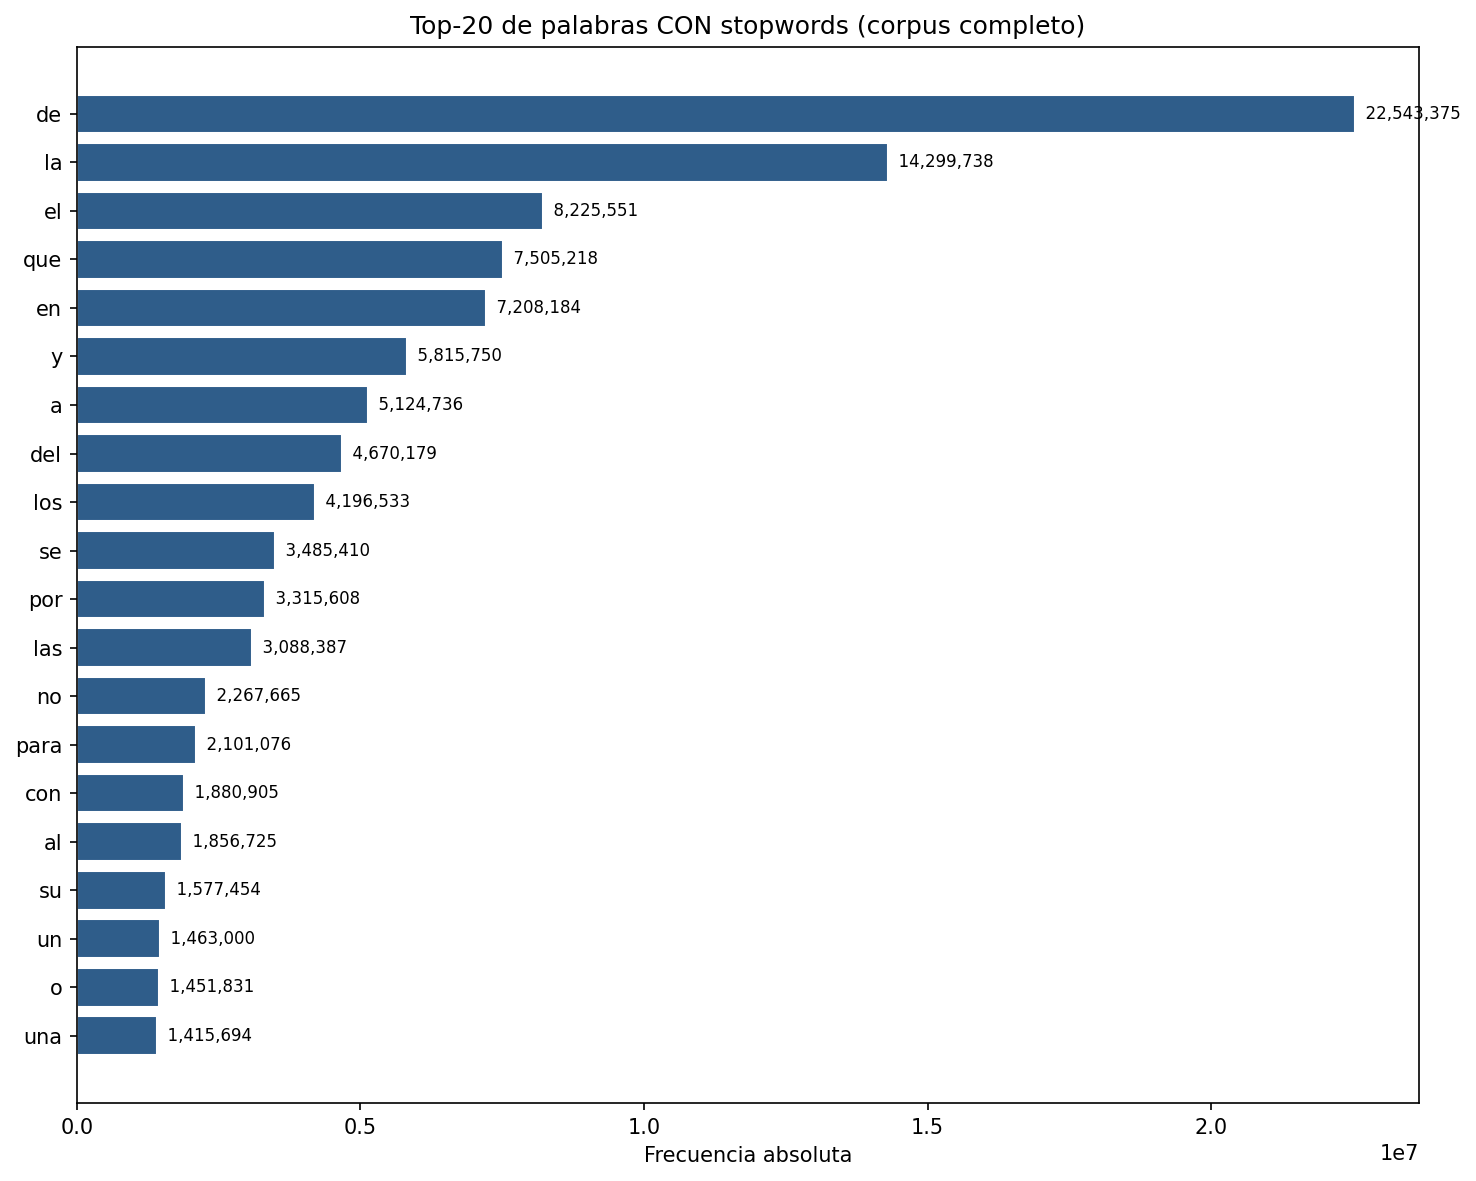
\includegraphics[width=\linewidth]{fig_top20_con_stopwords.png}
        \caption{Con palabras vacías gramaticales.}
        \label{fig:top20_con}
    \end{subfigure}%
    \hfill
    \begin{subfigure}[t]{0.48\linewidth}
        \centering
        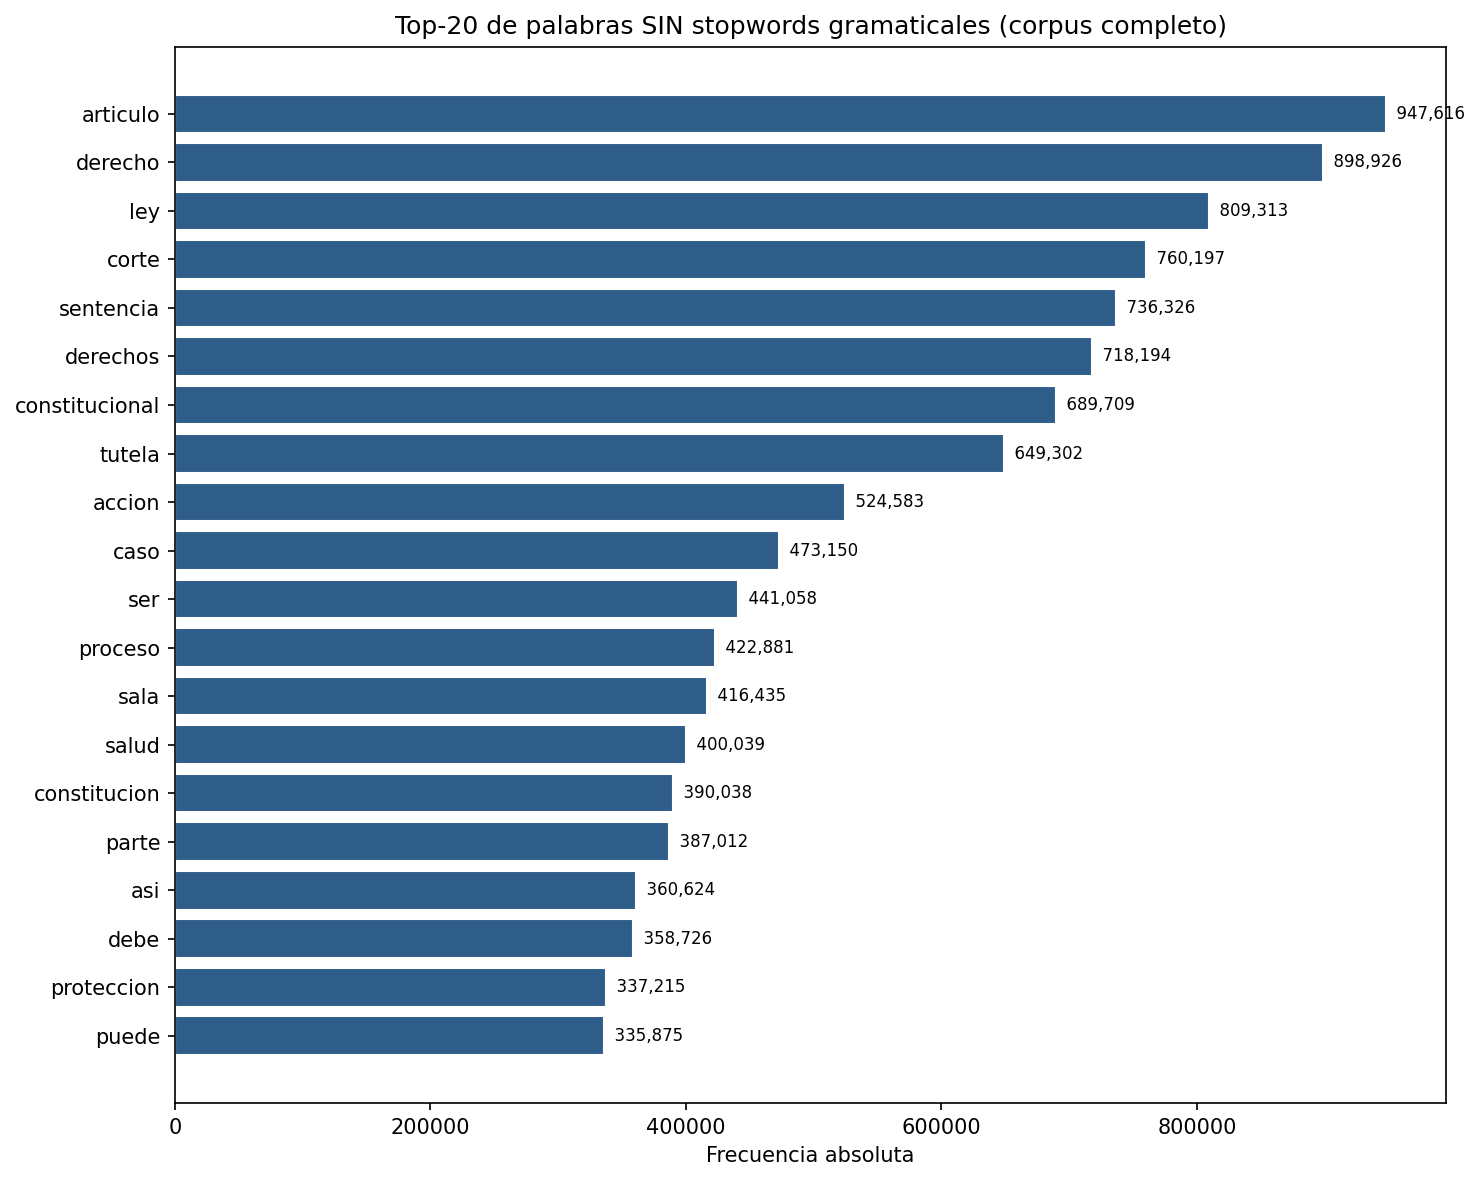
\includegraphics[width=\linewidth]{fig_top20_sin_stopwords.png}
        \caption{Sin palabras vacías gramaticales.}
        \label{fig:top20_sin}
    \end{subfigure}
    \caption{Top-20 de palabras más frecuentes del corpus completo (23.742 sentencias).}
    \label{fig:top20}
\end{figure}

\subsection{Distribución temporal}
La figura \ref{fig:por_anio} muestra el número de sentencias por año de emisión. El volumen es relativamente estable en torno a 950--990 providencias anuales entre 1999 y 2014, desciende progresivamente entre 2015 (763) y 2020 (505) y colapsa en 2021 a 20 documentos, evidencia de que la cobertura de 2021 es parcial y de que el nombre del archivo (que sugiere 2022) no corresponde con el contenido real. Por tipo de providencia, las sentencias de tutela dominan el corpus (72,0\,\% del total), seguidas por las de constitucionalidad (26,3\,\%) y las de unificación (1,7\,\%).

\begin{figure}[ht]
    \centering
    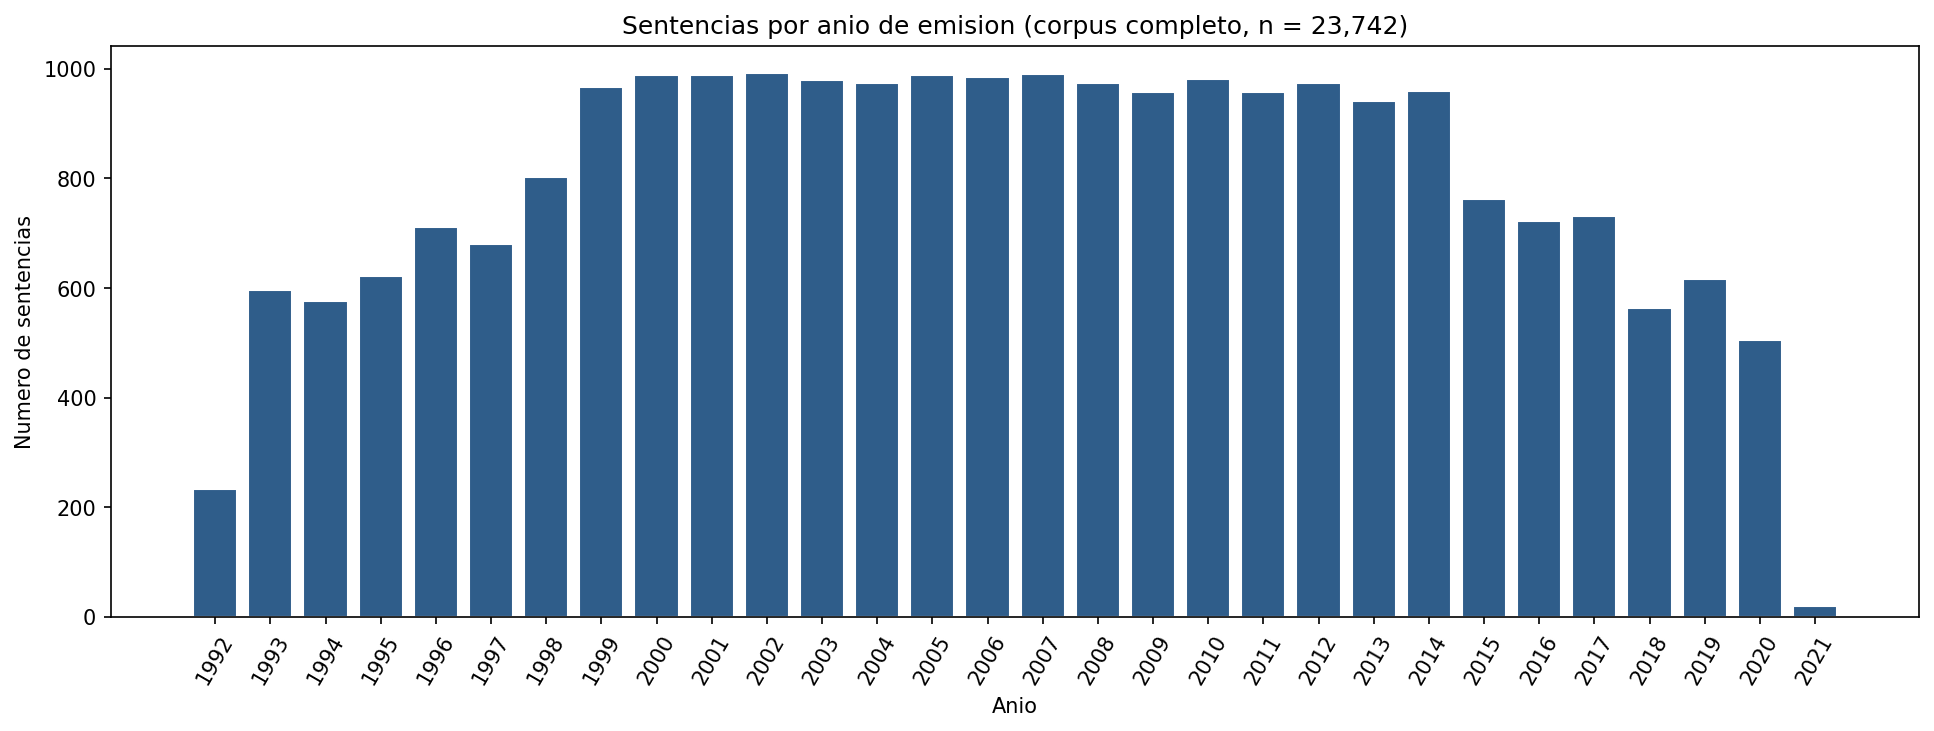
\includegraphics[width=0.9\linewidth]{fig_sentencias_por_anio.png}
    \caption{Sentencias del corpus por año de emisión, 1992--2021.}
    \label{fig:por_anio}
\end{figure}

\subsection{Nubes de palabras por año}
La figura \ref{fig:nubes} agrega el corpus completo en nubes de palabras anuales (una nube por año con los 1.000 términos más frecuentes de ese año). Para que el contenido temático sea visible, además de las 306 stopwords gramaticales se excluyeron 65 formas de vocabulario jurídico-procesal propio del género: \emph{sentencia(s)}, \emph{corte}, \emph{constitucional}, \emph{derecho(s)}, \emph{justicia}, \emph{tribunal}, \emph{magistrado(s)}, \emph{ponente}, \emph{demanda(s)}, \emph{expediente(s)}, \emph{colombia}, \emph{bogota}, \emph{republica}, \emph{accion(es)}, \emph{tutela(s)}, \emph{articulo(s)}, \emph{ley(es)}, \emph{norma(s)}, \emph{proceso(s)}, \emph{providencia(s)}, \emph{sala}, \emph{parte(s)}, entre otras. El año 2021 se excluyó por tener menos de 50 documentos (criterio de agregación), y la figura se presenta en tres paneles (1992--2001, 2002--2011 y 2012--2020) para conservar la legibilidad. La lectura cualitativa de las nubes permite apreciar la estabilidad de las fórmulas del género; el análisis cuantitativo de la evolución léxica por periodos se abordará en la entrega 2.

\begin{figure}[ht]
    \centering
    \begin{subfigure}[b]{0.46\linewidth}
        \centering
        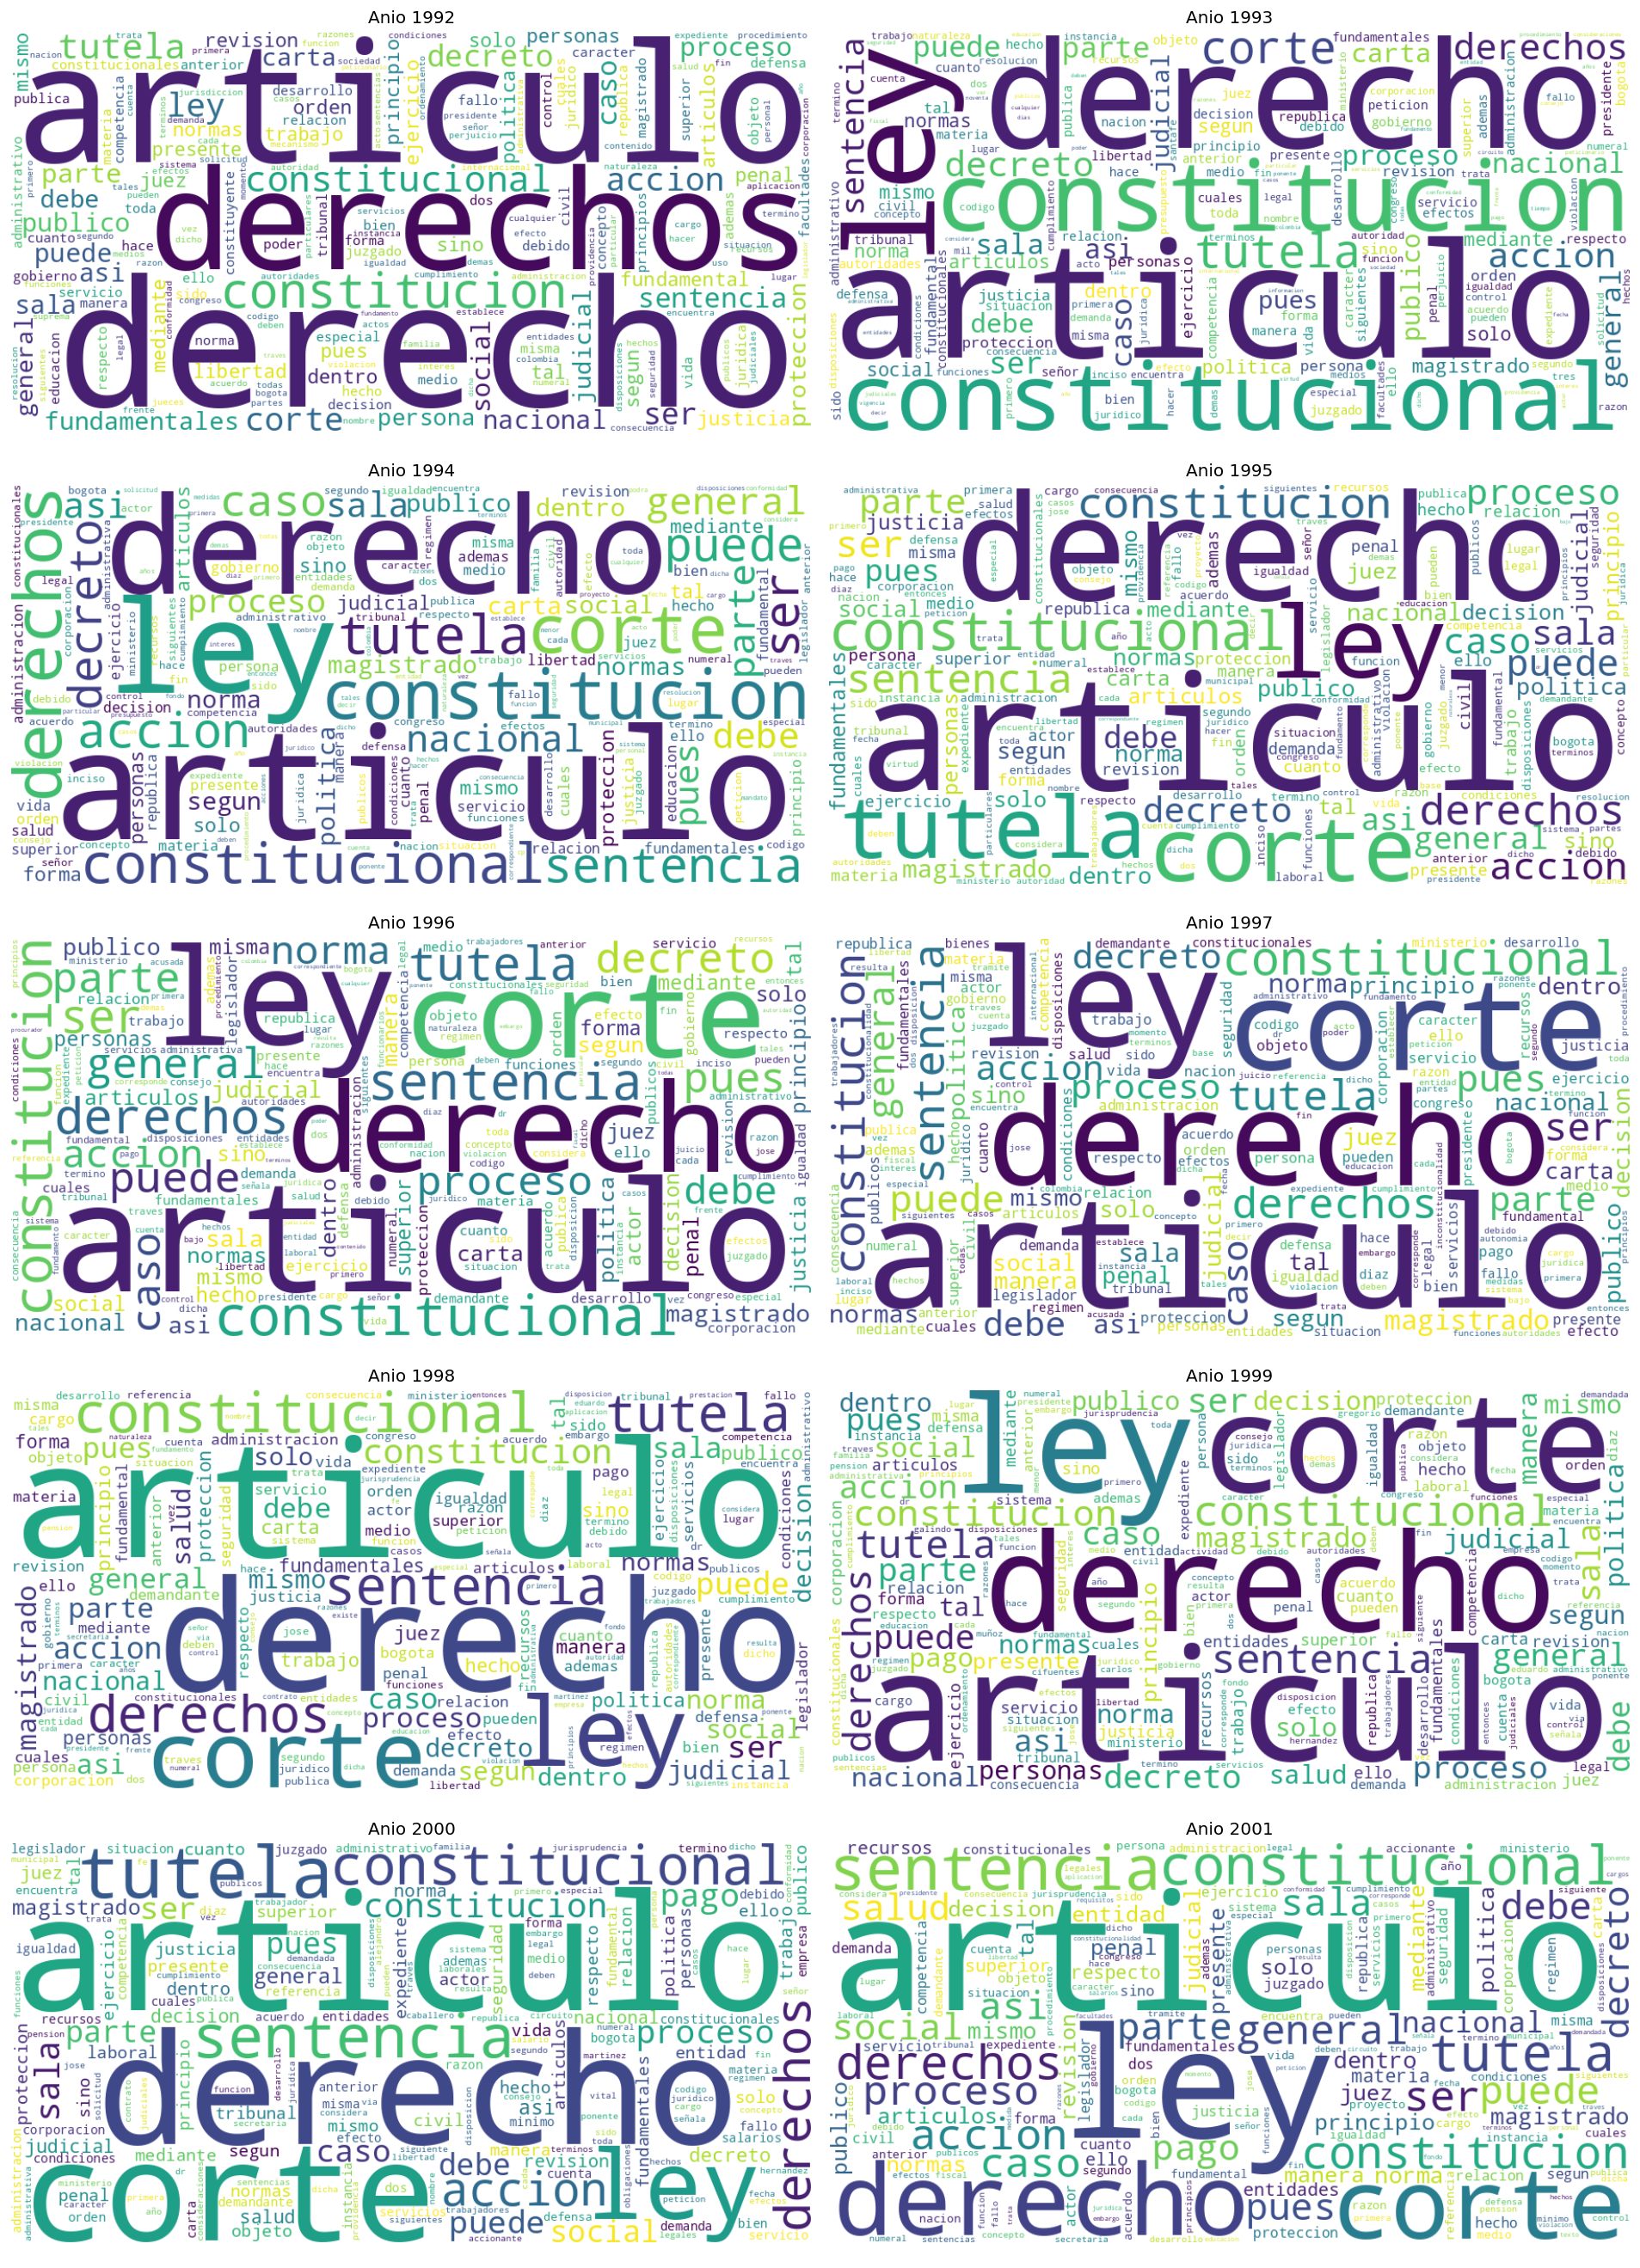
\includegraphics[width=\linewidth]{fig_nubes_por_anio_1992_2001.png}
        \caption{Nubes anuales 1992--2001.}
        \label{fig:nubes_1}
    \end{subfigure}%
    \hfill
    \begin{subfigure}[b]{0.46\linewidth}
        \centering
        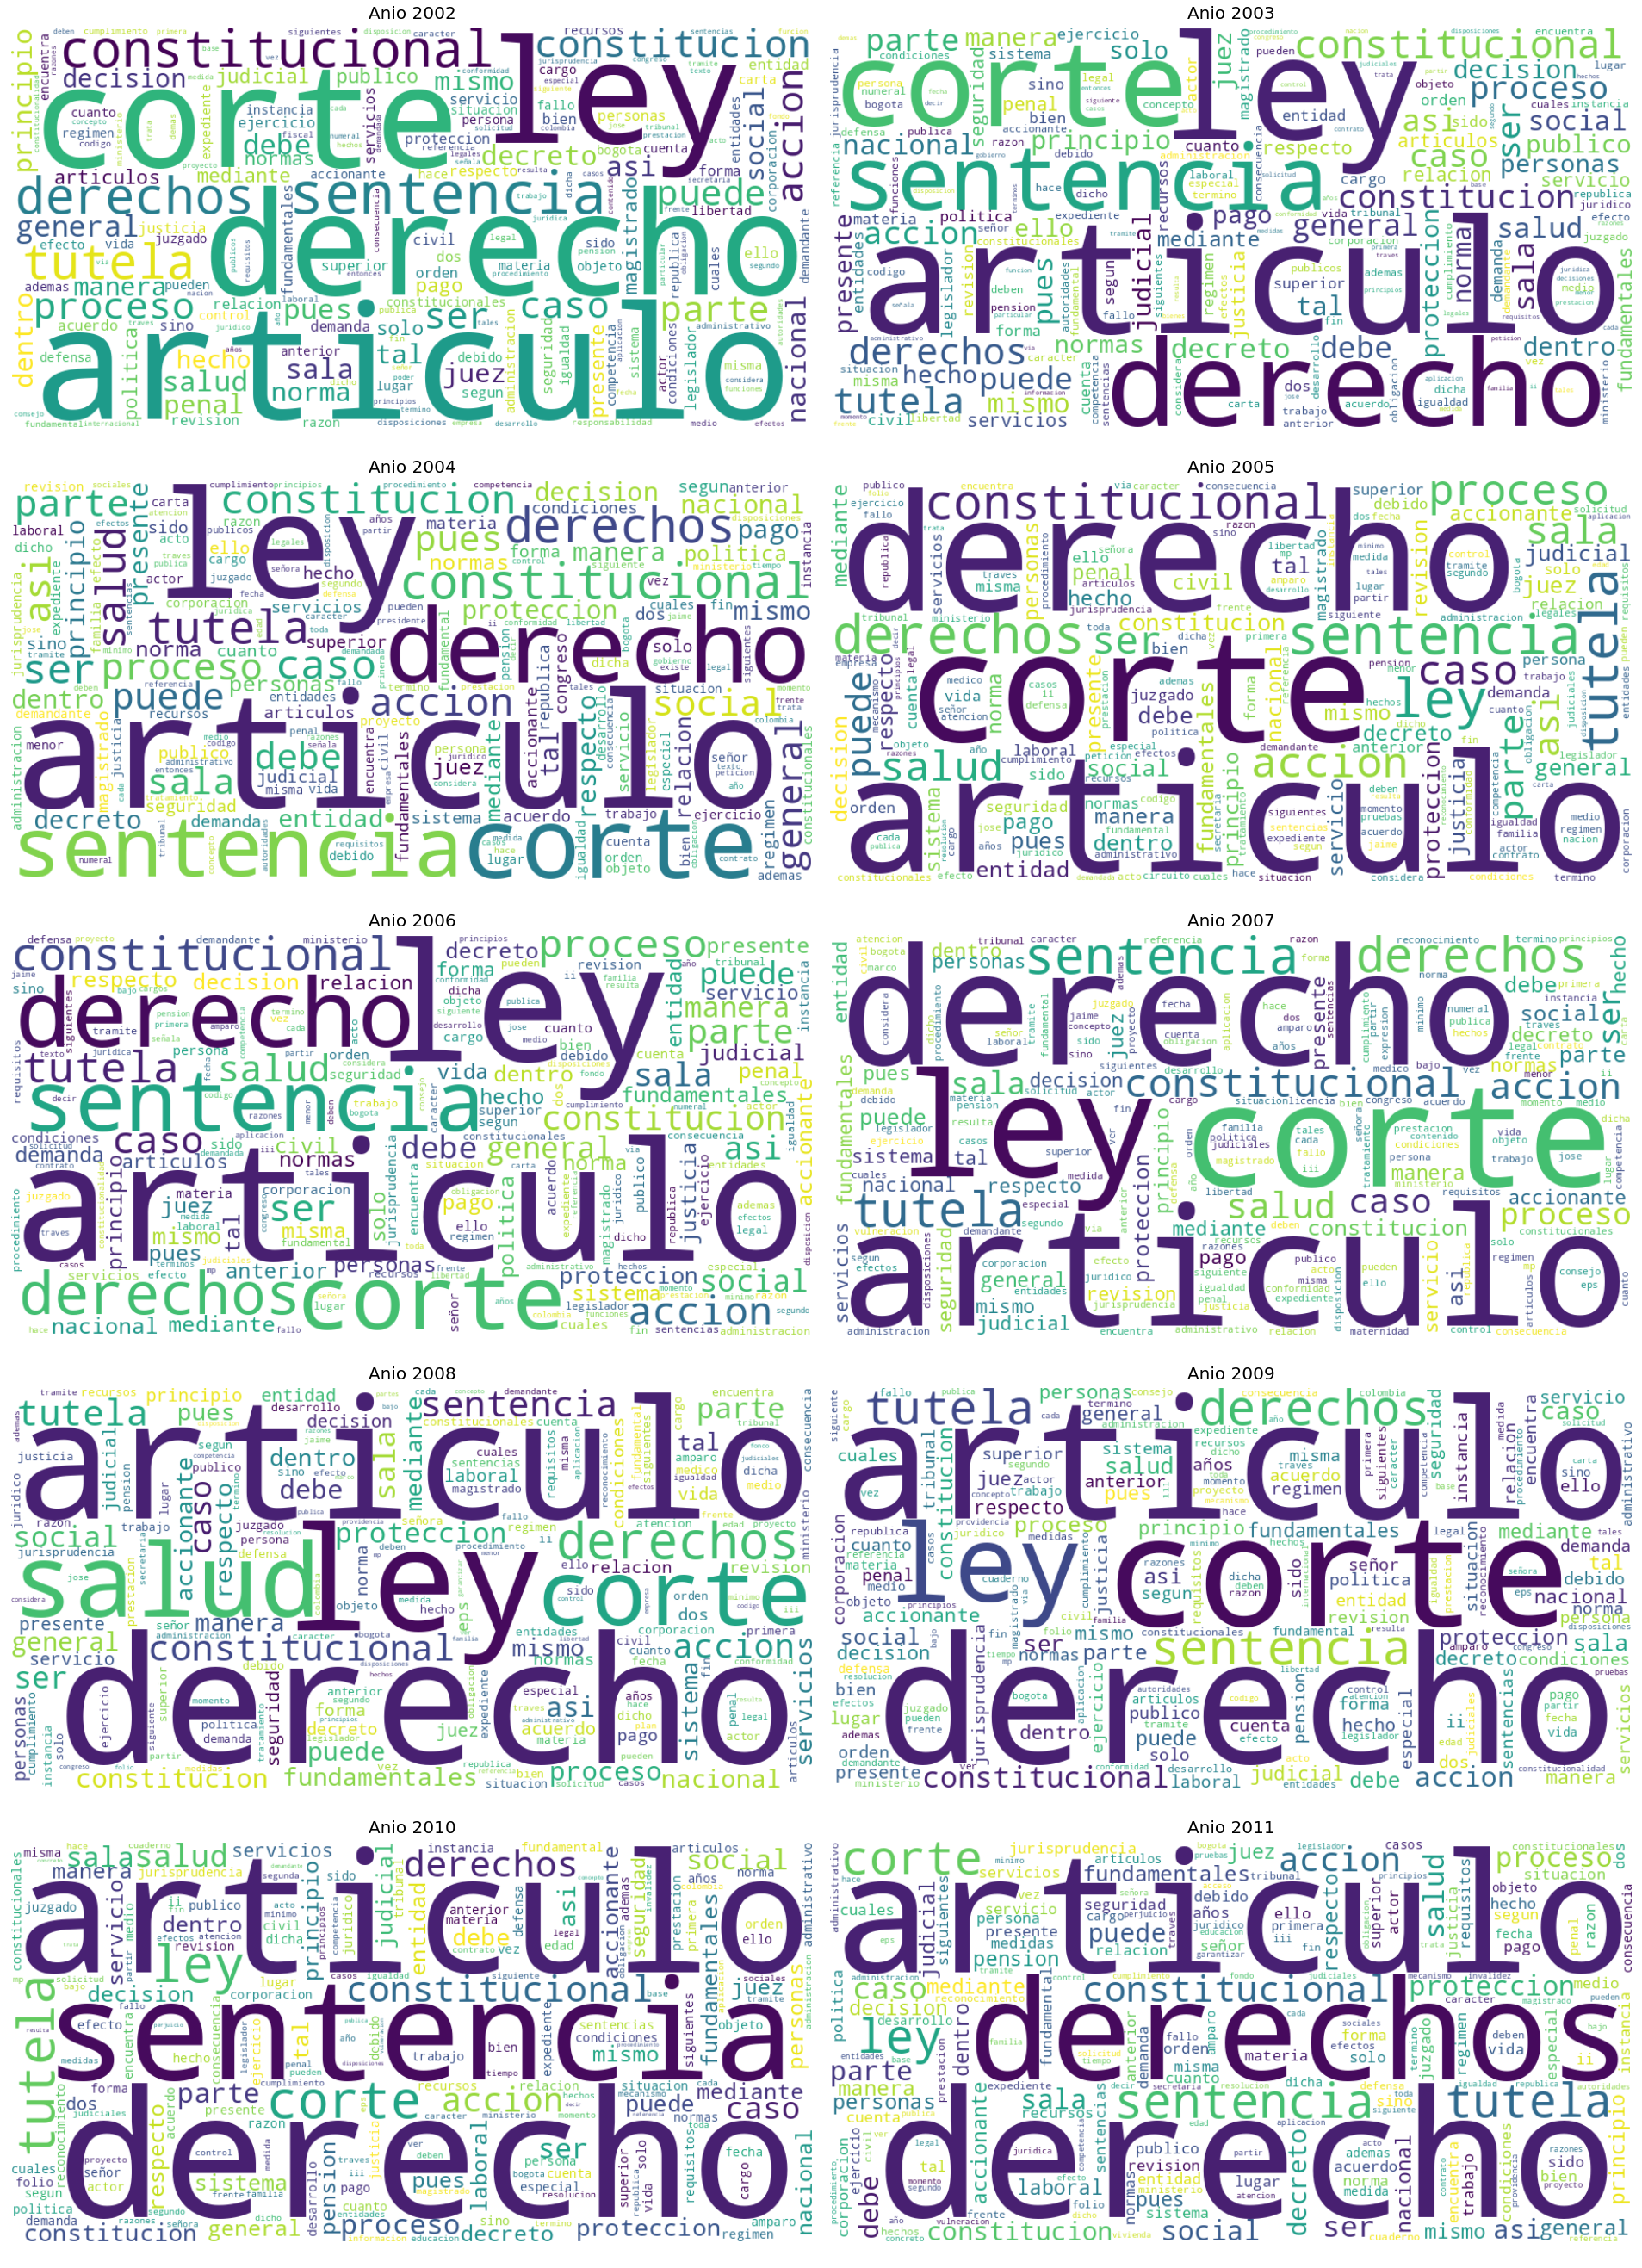
\includegraphics[width=\linewidth]{fig_nubes_por_anio_2002_2011.png}
        \caption{Nubes anuales 2002--2011.}
        \label{fig:nubes_2}
    \end{subfigure}
    \caption{Nubes de palabras por año (sin stopwords gramaticales ni de dominio jurídico).}
    \label{fig:nubes}
\end{figure}

\begin{figure}[ht]
    \centering
    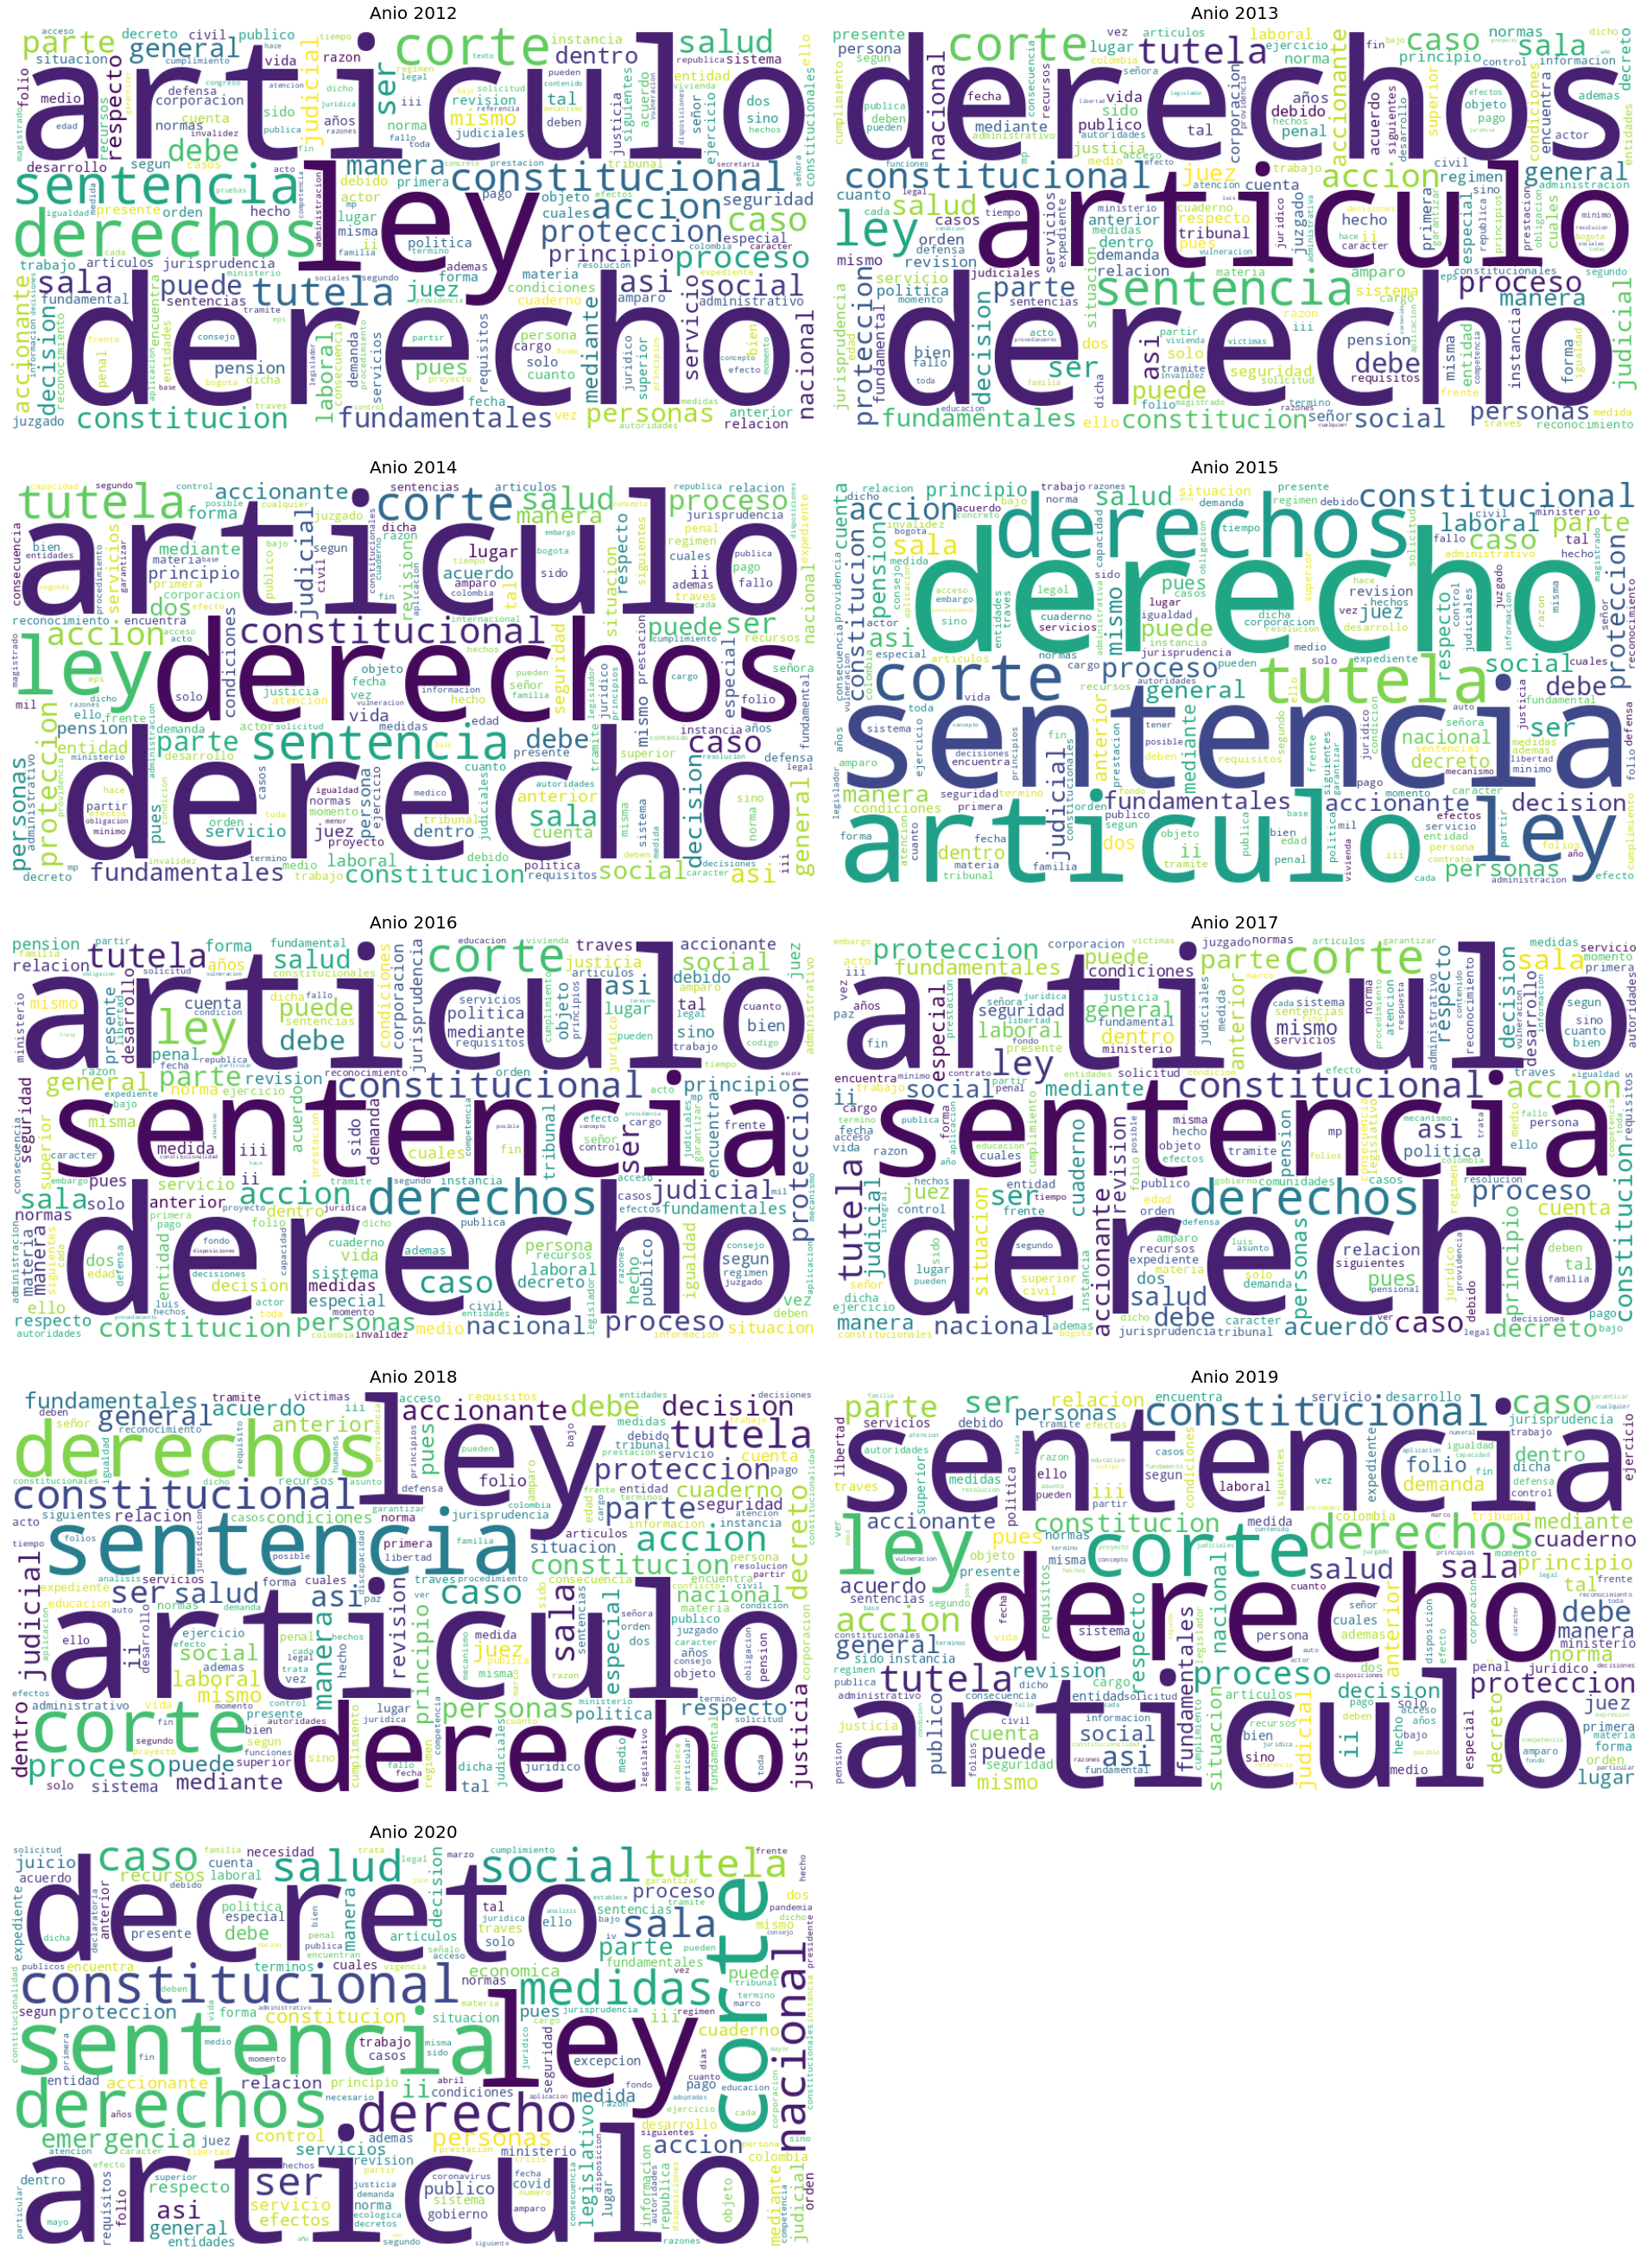
\includegraphics[width=0.46\linewidth]{fig_nubes_por_anio_2012_2020.png}
    \caption{Nubes de palabras anuales 2012--2020 (continuación de la figura \ref{fig:nubes}).}
    \label{fig:nubes_3}
\end{figure}

% =====================================================================
% SECCION 4: ESTADO DEL ARTE
% =====================================================================
\section{Estado del arte y antecedentes}
La búsqueda bibliográfica (realizada el 2026-09-05 en arXiv, Semantic Scholar, OpenAlex, Crossref y el propio Hugging Face) no encontró trabajos indexados que usen el \emph{dataset} exacto de este proyecto \cite{manuel2022sentencias}; sí existen antecedentes sólidos sobre su corpus subyacente y sobre la metodología. Anzola Cortés aplicó minería de datos a más de 6.000 sentencias de constitucionalidad de la Corte Constitucional colombiana (1992--2020), el mismo universo documental del repositorio, y documentó los problemas estructurales típicos de estos textos (fórmulas de estilo y referencias embebidas) \cite{anzolaCortes2021algoritmos}. Barbosa Becerra analizó léxico-discursivamente sentencias de la propia Corte y evidenció la estabilidad de sus fórmulas y la existencia de un léxico jurídico especializado, lo que justifica ampliar las stopwords gramaticales con términos jurídico-procesales \cite{barbosaBecerra2021comportamiento}.

En cuanto a métodos, HaCohen-Kerner y colaboradores mostraron empíricamente que la elección del preprocesamiento (minúsculas, números, stopwords, normalización, etc.) cambia los resultados de clasificación según el corpus y la tarea \cite{hacohenKerner2020influence}; por ello esta entrega documenta cada paso de limpieza y aplica la misma normalización al corpus y a la lista de stopwords. González-González y colaboradores presentan un \emph{pipeline} de clasificación de sentencias judiciales en español con diccionarios de dominio construidos con expertos legales \cite{gonzalezGonzalez2023automatic}, y Soh y colaboradores estudiaron corpus de sentencias largas y advierten sobre la cautela necesaria al reportar frecuencias globales dominadas por las plantillas \cite{soh2019legalarea}.

Para la dimensión temporal, Raj y colaboradores demuestran con análisis de corpus y pruebas estadísticas que el vocabulario y la extensión de las sentencias cambian de forma medible tras reformas normativas, lo que respalda el análisis por año \cite{raj2026collective}; Aletras y colaboradores mostraron, en el ámbito del Tribunal Europeo de Derechos Humanos, el poder predictivo de distintas secciones de las sentencias con NLP clásico \cite{aletras2016predicting}. En el plano de los modelos, Chalkidis y colaboradores introdujeron LEGAL-BERT y mostraron que el vocabulario jurídico difiere del general, lo que motiva evaluar adaptación de dominio en las fases siguientes \cite{chalkidis2020legalbert}, y Löffler y colaboradores evidencian la escasez de recursos legales anotados en español para Latinoamérica \cite{loffler2025predicting}. En síntesis: los conteos sobre el corpus completo (y no sobre muestras), el contraste con/sin stopwords, la normalización sin tildes y el análisis temporal adoptados en esta entrega se apoyan directamente en estos antecedentes.

% =====================================================================
% SECCION 5: CONCLUSIONES
% =====================================================================
\section{Conclusiones y trabajo futuro}
En esta entrega se consolidó el corpus de análisis: 23.742 sentencias de la Corte Constitucional de Colombia (1992--2021) depuradas a partir de las 23.750 filas del repositorio, con una tasa de extracción de identificador y año del 99,97\,\% y 8 exclusiones documentadas (6 autos y 2 fragmentos HTML). Sobre el corpus completo se ejecutó un \emph{pipeline} de limpieza reproducible (normalización sin tildes que preserva la \emph{ñ}, filtrado alfabético y stopwords normalizadas), se calcularon las medidas textuales reales (260.988.316 palabras crudas; $\approx$ 10.993 por documento) y se generaron las figuras de frecuencias, distribución temporal y nubes anuales. Los resultados confirman el carácter extenso y formulaico del género y el dominio del léxico jurídico-procesal, y dejan evidencia medible para las siguientes fases.

El trabajo futuro (entrega 2) comprende: (i) lematización y etiquetado POS con \emph{spaCy} para agrupar flexiones; (ii) representaciones del texto (TF-IDF y vectores densos) y análisis de diversidad léxica por año y por tipo de providencia; (iii) experimentos de clasificación automática por tipo y temática, contrastando modelos clásicos con modelos de lenguaje de dominio legal como LEGAL-BERT \cite{chalkidis2020legalbert}; y (iv) la evaluación de estrategias de resumen automático para sentencias extensas. La textometría aquí reportada, con cifras sobre el corpus completo y decisiones metodológicas documentadas, es la línea base de esas etapas.

% =====================================================================
% BIBLIOGRAFIA (estilo apalike; todas las claves citadas existen en
% references.bib y todas las entradas del .bib se citan en el texto)
% =====================================================================
\bibliographystyle{apalike}
{\small\bibliography{references}}

\end{document}
